\subsection{Performances matérielles}
\subsubsection{Stockage de données}
\noindent Pour tester les performances de la microSD et du disque SDD interne M.2 NVMe, l'utilitaire "hdparm" peut être facilement utilisé. 
{
   \vspace{0.1em} % Adjust the height of the space between caption and tabular
   \renewcommand*{\arraystretch}{1.4}
   \begin{longtable}[t]{@{}|p{28em}|p{2em}|p{2em}|p{3em}|@{}} 
      \caption{Comparaison des performances du "data read" entre un SDD M.2 NVMe et une microSD}\label{tab:Timing O_DIRECT disk reads}\\
      \hline
      \textbf{Disk reads} & \textbf{MB} & \textbf{sec} & \textbf{MB/sec}\\
      \hline
      Samsung 970 EVO Plus 250GB M.2 NVMe Internal Solid State Drive & 1004 & 3 & 334.15\\
      \hline
      microSD Scan Disk Ultra 32Gb HC I Class 10 & 122 & 3.03 & 40.22\\
      \hline
      microSD Samsung EVO 64Gb Plus XC I Grade 3 Class 10 & 256 & 3.02 & 84.71\\
      \hline
      microSD Samsung EVO 64Gb Select XC I Grade 3 Class 10 & 92 & 3.01 & 30.54\\
      \hline
   \end{longtable}
}
\subsubsection{Performances système}
\noindent Les diagrammes suivants présentent l'état du nano-ordinateur avant la segmentation, pendant et après. Les indicateurs qui sont observés sont ceux de la mémoire, la fréquence, le I/O, la consommation, la température. Afin de montrer l'impacte potentiel de l'application Chromium, elle est démarrée entre deux segmentations, et pendant la segmentation. 
\vspace{\baselineskip}
\\
\noindent La carte microSD "Scan Disk Ultra 32Gb class 10 HC I" a été utilisée pour les tests de performance système. La carte microSD "Samsung EVO 64Gb Plus class 10 HC I" n'était malheureusement plus fonctionnelle au moment des tests, celle-ci ayant été réservée pour tenter d'adapter l'architecture aux images terrain locales. 
\vspace{\baselineskip}
\\
\noindent Le test infère en temps réel la vidéo qui est capturée avec la caméra du nano-ordinateur. Le réseau \acrshort{fcn} qui est utilisé est celui fournit par NVIDIA "fcn-resnet18-deepscene-576x320". Ce modèle détecte automatiquement la résolution la plus appropriée avec cette caméra, c'est-à-dire 30 images par seconde (\acrshort{fps}) et une résolution de 1280x720. Le test dure 1400 secondes, un peu de plus de 23 minutes. Il peut se diviser en onze périodes d'observation, qui sont brièvement décrites ci-dessous: 
\begin{enumerate}
   \item La première période est celle entre la 1re seconde et la 200e seconde, et qui permet d'observer l'état du système au démarrage du nano-ordinateur sans opération mise à part celle de la collecte des statistiques. 
   \item La seconde période est entre la 200e seconde et la 400e, et qui correspond à la première segmentation avec la caméra. Elle permet d'observer le système lors du premier démarrage de la segmentation. 
   \item La troisième période est celle entre la 400e seconde et le premier démarrage de Chromium. Elle permet d'observer la réaction du système après l'arrêt de la segmentation. 
   \item La quatrième période est celle entre le premier démarrage de Chromium et son arrêt. Elle permet d'observer le comportement du système lors de l'utilisation de Chromium, qui est suspecté de ralentir le système, lorsqu'actif (observations faites durant l'essai).
   \item La cinquième période est celle entre l'arrêt de Chromium et le démarrage de la seconde segmentation avec la caméra. Cette période permet d'observer la réaction du système après l'arrêt de Chromium. 
   \item La sixième période est celle entre le démarrage de la seconde segmentation avec la caméra et son arrêt. Cette période permet d'observer la réaction du système pendant la seconde segmentation. 
   \item La septième période est celle entre l'arrêt de la seconde segmentation et le démarrage de la troisième segmentation avec la caméra. Elle permet d'observer la réaction du système après l'arrêt de la segmentation la seconde fois. 
   \item La huitième période est celle entre le démarrage de la troisième segmentation et le démarrage de Chromium la seconde fois. Cette période permet d'observer la réaction du système pendant le démarrage de la segmentation la troisième fois. 
   \item La neuvième période est celle entre le deuxième démarrage de Chromium et son arrêt. Elle permet d'observer le comportement du système lors de l'utilisation de Chromium pendant l'inférence.
   \item La dixième période est celle entre l'arrêt Chromium la seconde fois et l'arrêt de la troisième segmentation. Cette période permet d'observer la réaction du système après l'arrêt de Chromium pendant l'inférence. 
   \item La onzième période est celle entre l'arrêt de la troisième segmentation et l'arrêt du test et de la collecte des statistiques. Elle permet d'observer la réaction du système après l'arrêt de la segmentation la troisième fois. 
\end{enumerate} 
\begin{figure}[H]
   \centering
   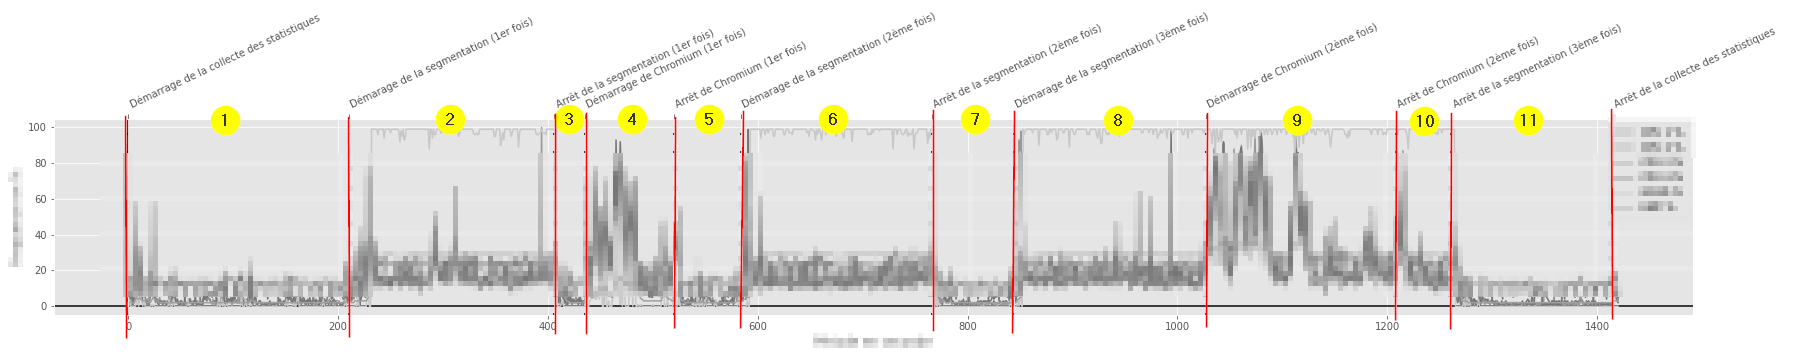
\includegraphics[width=1.0\textwidth]{test_periods}
   \caption{Les périodes du diagramme des performances système}
   \label{fig:test_periods}
\end{figure}
{
   % \clearpage 
   % \newpage
   \begin{landscape}
   \begin{figure}[H]
      \centering
      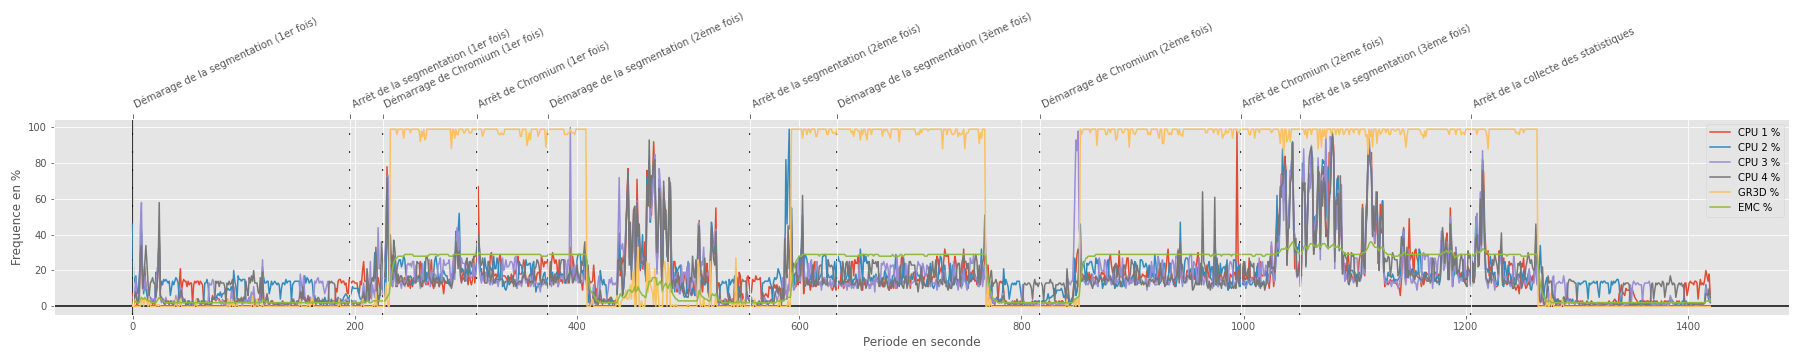
\includegraphics[width=1.5\textwidth]{frequency_usage}
      \caption{Diagramme des performances système: la fréquence}
      \label{fig:frequency_usage}
   \end{figure}
   \begin{figure}[H]
      \centering
      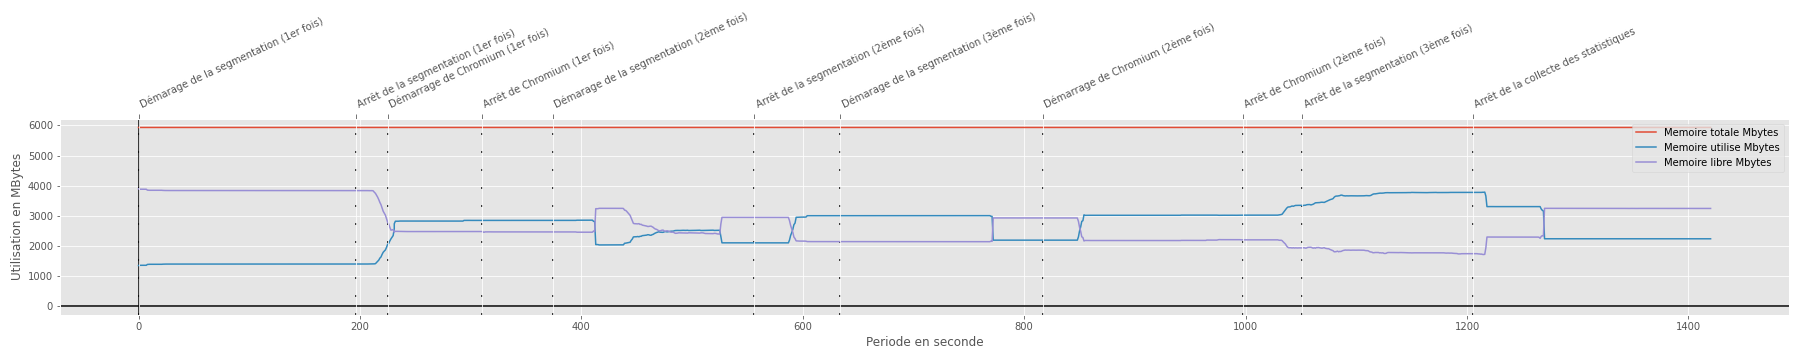
\includegraphics[width=1.5\textwidth]{memory_usage}
      \caption{Diagramme des performances système: la mémoire}
      \label{fig:memory_usage}
   \end{figure} 
   \begin{figure}[H]
      \centering
      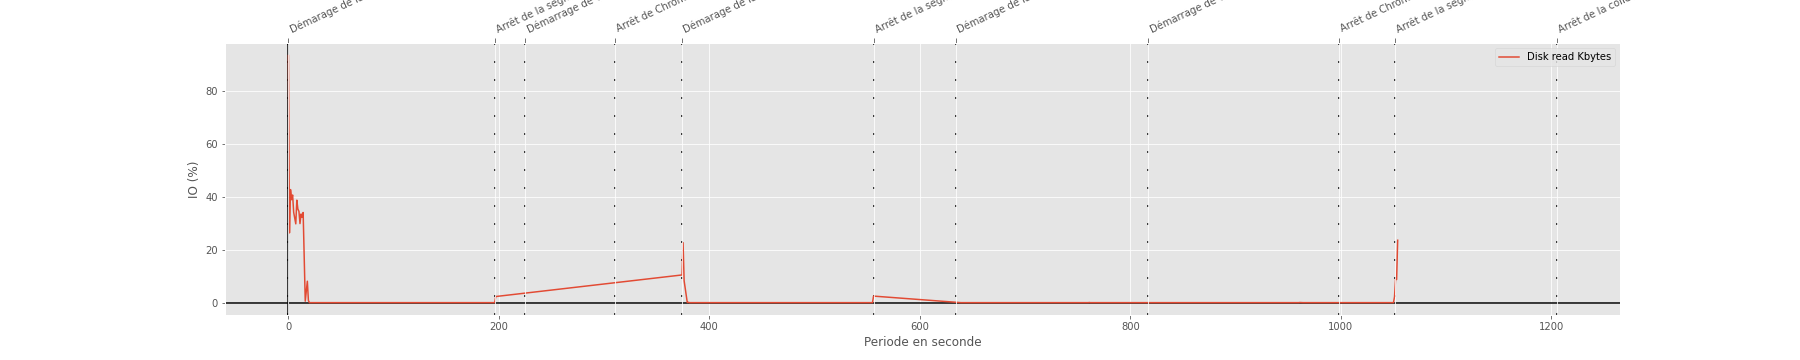
\includegraphics[width=1.5\textwidth]{io}
      \caption{Diagramme des performances système: le I/O total en \% de la segmentation}
      \label{fig:io}
   \end{figure}
   \begin{figure}[H]
      \centering
      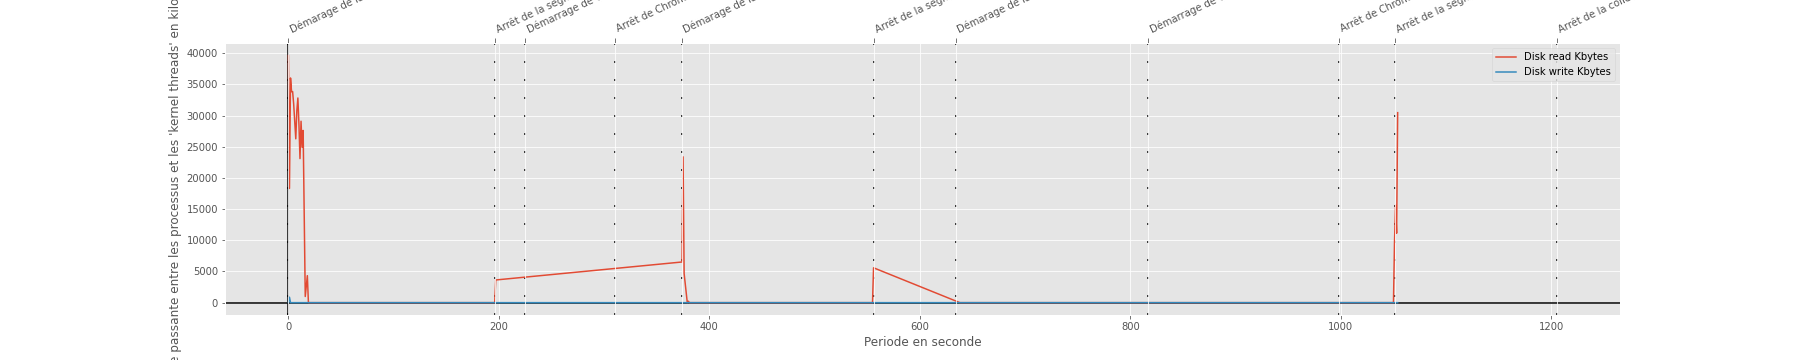
\includegraphics[width=1.5\textwidth]{io_segnetcamera}
      \caption{Diagramme des performances système: le I/O en KBytes de la segmentation}
      \label{fig:io_segnetcamera}
   \end{figure} 
   \begin{figure}[H]
      \centering
      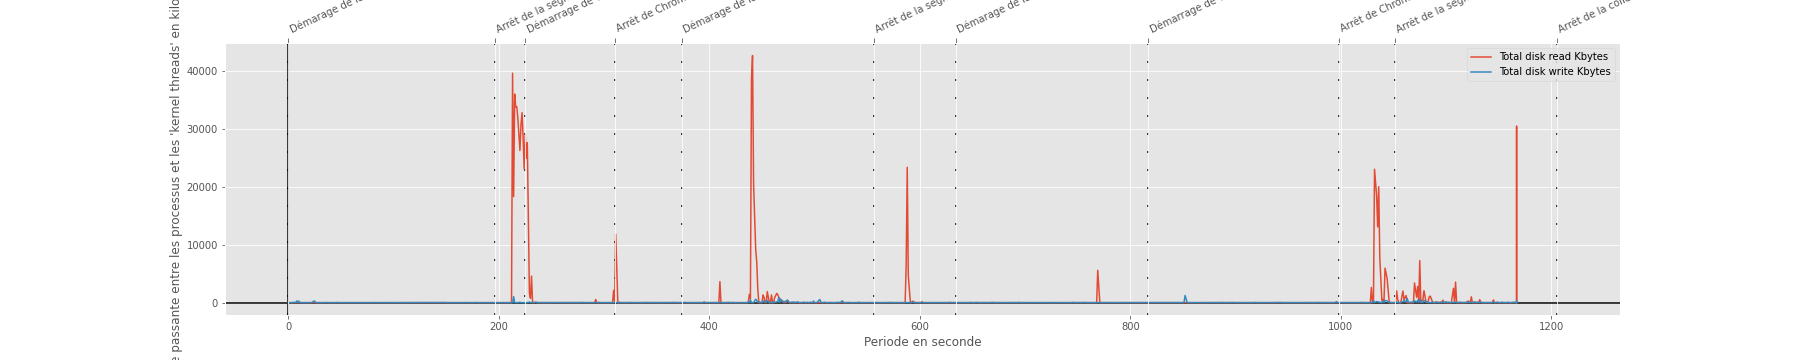
\includegraphics[width=1.5\textwidth]{io_totaldisk}
      \caption{Diagramme des performances système: le I/O total du disque en KBytes}
      \label{fig:io_totaldisk}
   \end{figure} 
   \begin{figure}[H]
      \centering
      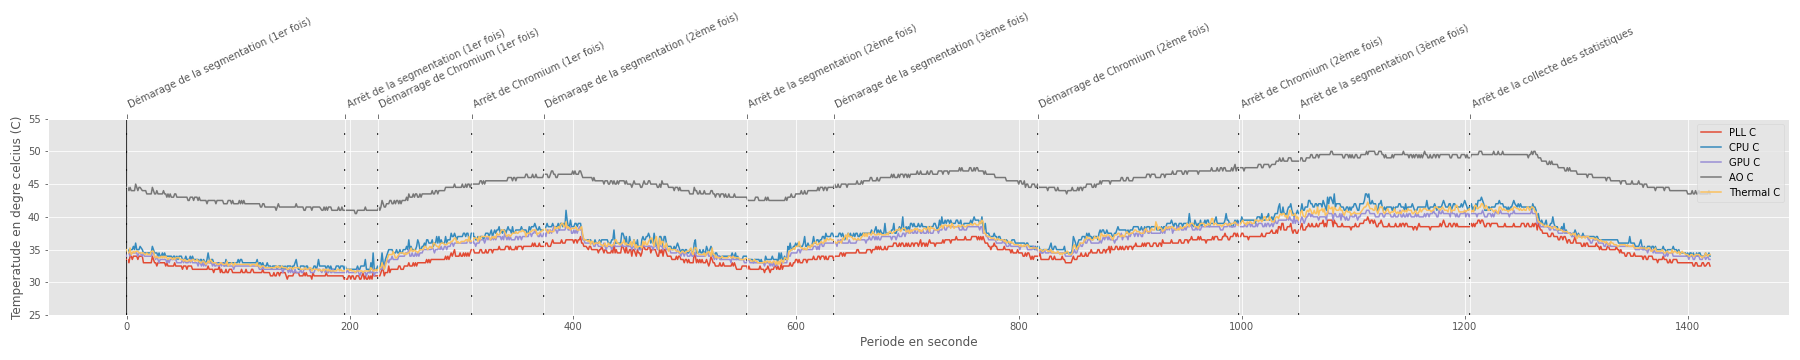
\includegraphics[width=1.5\textwidth]{temperature}
      \caption[Diagramme des performances système: les températures]{Diagramme des performances système: les températures\protect\footnotemark}
      \label{fig:temperature}
   \end{figure} 
   \footnotetext{PLL: Phase locking loop thermal sensor; AO: Always on thermal sensor. \url{https://forums.developer.nvidia.com/t/operating-temperature-range-on-jetson-nano/73555/10}}
   \begin{figure}[H]
      \centering
      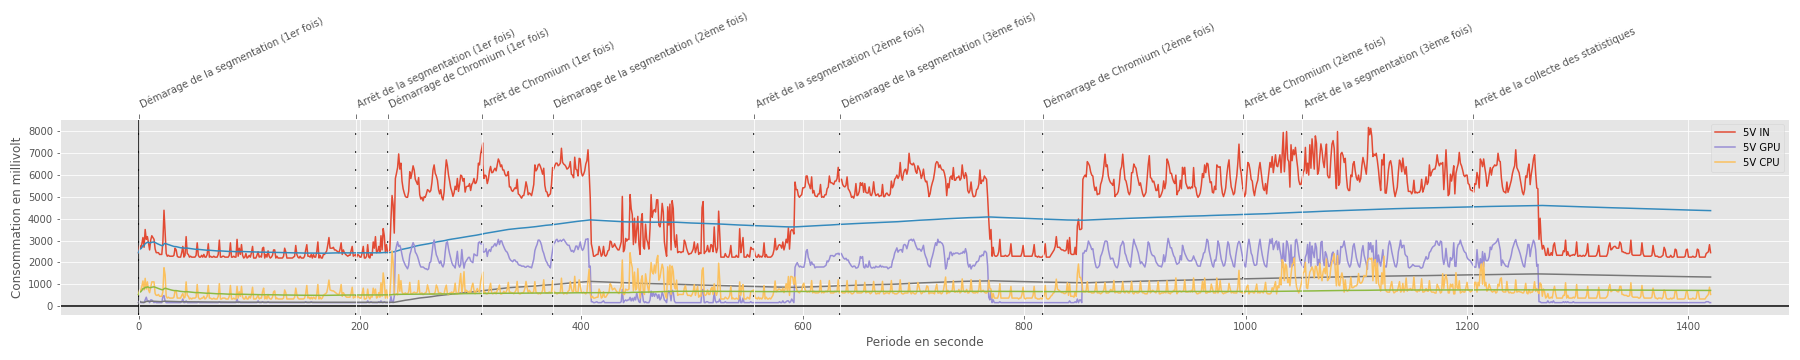
\includegraphics[width=1.5\textwidth]{consommation}
      \caption{Diagramme des performances système: la consommation}
      \label{fig:consommation}
   \end{figure}
   \end{landscape}
   % \clearpage
   % \newpage
}
\subsection{Performances de l'inférence}
\subsubsection{Images}
\noindent Les tests ont été faits avec l'architecture "fcn-resnet18-deepscene-576x320" fourni par NVIDIA. 
\vspace{\baselineskip}
\\
\noindent Lors de l'entrainement et l'inférence, le script montre un \acrshort{iou} moyen de 75 \%. Mais l'objet d'intérêt de l'essai n'est pas la qualité de la segmentation de l'image complète, mais seulement de la piste cyclable. Certains efforts ont dû être dépensés\footnote{\url{https://github.com/vince7lf/vince7lf.github.io/blob/master/_notebooks/2020-06-21-image_pred_color.ipynb}} afin de pouvoir observer le \acrshort{iou} et le F1 score de la segmentation sémantique de la piste cyclable uniquement.
\vspace{\baselineskip}
\\
\noindent Le résultat de la segmentation sémantique peut-être visualisé avec ces deux photos, prises du jeu de donnée de test de la forêt de Freiburg et utiliser comme jeu de données de test pour l'architecture. L'image utilisée possède une version vérité terrain (\acrshort{gt}). L'image générée est l'image prédite et peut être comparée avec l'image vérité terrain (\acrshort{gt}), tant que la palette de couleur est identique à la version vérité terrain (\acrshort{gt}). 
\vspace{\baselineskip}
\\
\noindent Il s'avère que le \acrshort{iou} et F1 score sont assez élevés pour les deux photos pour la classe "Chemin". 
\begin{figure}[H]
   \centering
   {
      \tikz \fill [trail] (0.05, 0.05) rectangle (1.0, 0.5) ; {Chemin}
      \tikz \fill [grass] (0.05, 0.05) rectangle (1.0, 0.5) ; {Herbe}
      \tikz \fill [vegetation] (0.05, 0.05) rectangle (1.0, 0.5) ; {Végétation/arbres}
      \tikz \fill [sky] (0.05, 0.05) rectangle (1.0, 0.5) ; {Ciel}
      % \tikz \fill [obstacle] (0.05, 0.05) rectangle (1.0, 0.5) ; {Obstacle}
   }
   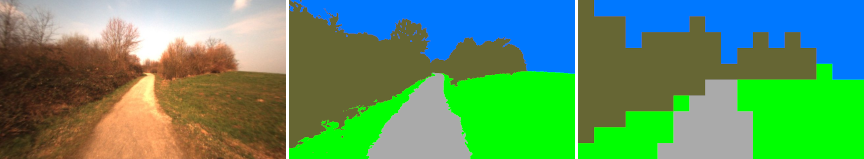
\includegraphics[width=1\textwidth]{b1-09517_Clipped_segmented}
   \caption[Segmentation sémantique de l'image b1-09517 générée par l'architecture]{(gauche) Image originale (b1-09517); (centre) vérité terrain (\acrshort{gt}); (droite) segmentation sémantique générée par l'architecture. Le \acrshort{iou} et le F1 score pour le chemin sont de +80 \%.}
   \label{fig:b1-09517_Clipped}
\end{figure}
\begin{figure}[H]
   \centering
   {
      \tikz \fill [trail] (0.05, 0.05) rectangle (1.0, 0.5) ; {Chemin}
      \tikz \fill [grass] (0.05, 0.05) rectangle (1.0, 0.5) ; {Herbe}
      \tikz \fill [vegetation] (0.05, 0.05) rectangle (1.0, 0.5) ; {Végétation/arbres}
      \tikz \fill [sky] (0.05, 0.05) rectangle (1.0, 0.5) ; {Ciel}
      \tikz \fill [obstacle] (0.05, 0.05) rectangle (1.0, 0.5) ; {Obstacle}
   }
   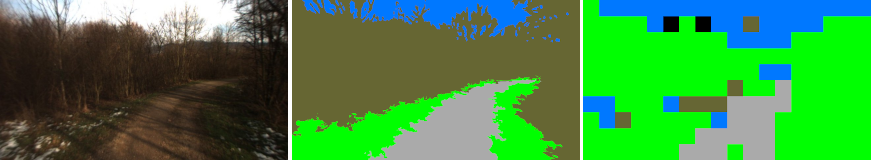
\includegraphics[width=1\textwidth]{b378-61_Clipped_segmented}
   \caption[Segmentation sémantique de l'image b378-61 générée par l'architecture]{(gauche) Image originale (b378-61); (milieu) vérité terrain (\acrshort{gt}); (droite) segmentation sémantique générée par l'architecture. Le \acrshort{iou} pour le chemin est +69 \%.}
   \label{fig:b378-61_mask}

\end{figure}
\subsubsection{Vidéos}
\noindent Il y a deux vidéos qui ont été utilisées pour tester les performances de la segmentation avec une vidéo. Comme il n'est pas évident de montrer une vidéo dans un essai, des liens sont mis à disposition. Ces vidéos sont disponibles dans le projet "Vision Météo" de Teams de l'Université de Sherbrooke. Chaque vidéo a été créée en filmant avec un téléphone intelligent l'écran du nano-ordinateur pendant que la segmentation est exécutée. Cela produit une vidéo HD 1080p 30 \acrshort{fps}. Lors de la seconde vidéo, les performances du système et les statistiques "tegrastats" sont affichées en plus de la segmentation.
\vspace{\baselineskip}
\\
\noindent J'ai tenté de capturer le résultat (vidéos/images) de l'inférence directement depuis le nano-ordinateur, mais ce n'est pas une bonne idée, car trop intrusif, l'inférence est ralentie. Deux images sont produites par l'architecture: "overlay" et "mask", qui sont directement rafraichies dans un XWindow. 
\begin{itemize}
   \item Lien\footnote{\url{https://usherbrooke.sharepoint.com/sites/ProjetVisionMto/Documents\%20partages/General/projet_visionmeteo/videos/gae724_lefv2603/resultats/20200221_020044.mp4}} vers une courte vidéo de 30 secondes démontrant l'inférence en temps réel de la segmentation sémantique d'une vidéo de la piste cyclable du pont Jacques-Cartier dans des conditions ensoleillées, mais avec un angle de vue qui change rapidement. Inférence effectuée en 30 \acrshort{fps} 1280x720 avec l'architecture "fcn-resnet18-deepscene-576x320";
   \item Lien\footnote{\url{https://usherbrooke.sharepoint.com/sites/ProjetVisionMto/Documents\%20partages/General/projet_visionmeteo/videos/gae724_lefv2603/resultats/20200412_232155.mp4}} vers une vidéo longue de +8 minutes présentant l'inférence en temps réel de la segmentation sémantique d'une vidéo d'une piste cyclable dans des conditions ensoleillée, mais mouillée, avec présence de neige. Durée de plus de 8 minutes. La taille de la vidéo est de 800Mb. La même vidéo, d'une durée de 30 secondes, est utilisée successivement avec différentes images par seconde (60 / 30 / 15 / 1 \acrshort{fps}) et résolutions (720x1280 / 480x640 / 320x480 / 240x320). L'architecture est "fcn-resnet18-deepscene-576x320". Selon le titre de la fenêtre xWindow présentant la segmentation, le \acrshort{fps} est autour de 23-26 \acrshort{fps}.
\end{itemize}
\vspace{\baselineskip}
\noindent Voici un tableau montrant les différentes résolutions et images par seconde (\acrshort{fps}) qui ont été testées avec l'architecture:
{
    \renewcommand*{\arraystretch}{1.4}
    \begin{table}[ht]
    \centering
    \caption{Résolutions et images par seconde (\acrshort{fps}) testés}\label{table:resolutions_tested}
    \vspace{0.1em} % Adjust the height of the space between caption and tabular
    \begin{tabular}{{@{}|p{35em}|@{}}}
         \hline
         \textbf{Résolutions qui fonctionnent}\\
         \hline
        320x576, 480x640, 720x1280, 768x1024, 768x1152, 800x1152, 832x1024, 864x1024\\
        \hline
        \textbf{Résolutions qui ne fonctionnent pas}\\
        \hline
        832x1120, 832x1152, 768x1280, 800x1280, 864x1152, 900x1152, 900x1280, 960x1600, 1080x1920, 1024x1024\\
        \hline
        \textbf{Images par seconde (\acrshort{fps}) supportées}\\
        \hline
        60/1, 30/1, 15/1, 1/1\\
        \hline
    \end{tabular}
    \end{table}
}
\subsection{Réentrainement}
\noindent Une tentative de réentrainement a été initiée. La première étape a été de vouloir regénérer le fichier \acrshort{onnx} tel que NVIDIA le fournit, sans autre effort de réentrainement. En effet les commandes fournies par NVIDIA pour segmenter une image ou une vidéo permettent de préciser une architecture personnalisée, tel que le fichier \acrshort{onnx}, les classes, les codes couleurs. L'idée est donc de bénéficier de cette possibilité. Le seconde étape était de créer un jeu de données adapté au contexte, c'est-à-dire avec des photos de différentes sections de pistes cyclables avec une qualité de surface variable (sèche, mouillée, avec neige, ensoleillé, ombragé, etc.), avec les images fournies par l'\acrshort{apcpontjc} et mon jeu personnel. Les difficultés attendues étaient d'uniformiser les résolutions des photos pour l'architecture SegNet18, mais surtout de créer des images vérités terrain (\acrshort{gt}), qui est beaucoup plus chronophage que difficile. Une fois le tout complété, la dernière étape est de re entrainé l'architecture SegNet18 avec ce jeu, et regénérer le nouveau fichier \acrshort{onnx}. 
\vspace{\baselineskip}
\\
\noindent Malheureuseument la première étape, de regénérer le fichier \acrshort{onnx}, ne s'est pas déroulé aussi simplement qu'espéré, et a remis en question la suite du réentrainement. La génération du fichier \acrshort{onnx} a tout d'abord réussie assez facilement, mais une erreur à l'exécution a remis en question l'intégrité de ce fichier. Une longue période d'investigation a débuté\footnote{\url{https://github.com/vince7lf/vince7lf.github.io/blob/master/_posts/2020-05-13-train-onnx-nano.md}}\footnote{\url{https://forums.developer.nvidia.com/t/trying-to-regenerate-onnx-for-jetson-nano/125494?u=vincelf}}, et finalement le fichier \acrshort{onnx} a pu être regénéré avec succès après la phase de réentrainement. Malheureusement le script fourni par NVIDIA qui adapte les photos du jeu de données de DeppScene pour le jeu d'entrainement et de test destiné au réentrainement de l'architecture SegNet18, génère des photos toutes noires, l'investigation s'est arrêtée à ce point.
